\subsection{Characterization of porous materials}

\subsubsection{BET surface area}\label{pyg:charac:betarea}

The BET surface area is one of the first standardised methods 
to calculate the surface area of a porous 
material~\cite{brunauerAdsorptionGasesMultimolecular1938}. 
It is generally applied on isotherms obtained through \ce{N2} 
adsorption at \SI{77}{\kelvin}, although other adsorbates 
(\ce{Ar} at \SI{77}{\kelvin} or \SI{87}{\kelvin}, 
\ce{Kr} at \SI{77}{\kelvin}, \ce{CO2} at \SI{293}{\kelvin})
have been used. In principle, any probe with an adsorption behaviour 
which can be described through the BET equation in the low pressure regime
can be used.

As mentioned before, the method assumes that the adsorption takes place 
on the surface of the material in incremental layers according to the
BET equation (\ref{pyg:eqn:bet}). 
Even if the adsorbent is porous, the initial amount adsorbed 
(usually between 0.05 - 0.4 \(p/p_0\)) can be
modelled through the equation written in its linear form:

\begin{equation}
    \frac{p/p_0}{n_{ads} (1-p/p_0)} = \frac{1}{n_{m} C} + \frac{C - 1}{n_{m} C}(p/p_0)
\end{equation}

If we plot the isotherm points as
\({(p/p_0)}/{n_{ads}(1-p/p_0)}\) versus \(p/p_0\), a linear region
can usually be found. The slope and intercept of this line
can then be used to calculate \(n_{m}\), the amount adsorbed at the
statistical monolayer, as well as \(C\), the BET constant.

\begin{align}
    n_{m} &= \frac{1}{s+i} & C &= \frac{s}{i} + 1
\end{align}

The surface area can then be calculated by using the moles
adsorbed at the statistical monolayer. If the specific area taken
by one of the adsorbate molecules on the surface is known, it is
inserted in the following equation together with Avogadro's number:

\begin{equation}
    a_{BET} = n_m A_N \sigma
\end{equation}

While a standard for surface area determinations, the BET area
should be used with care, as the assumptions made in
its calculation may not hold. To augment the validity of the BET
method, Rouquerol~\cite{rouquerolAdsorptionPowdersPorous2013} proposed
several checks to ensure that the BET region selected is valid:

\begin{itemize}

	\item The BET constant (\(C\)) obtained should be positive
    \item In the corresponding Rouquerol plot where \(n_{ads}(1-p/p_0)\)
    is plotted with respect to \(p/p_0\), the points chosen for BET
	analysis should be strictly increasing
	\item The loading at the statistical monolayer should be
	situated within the limits of the BET region

\end{itemize}

All these checks are implemented in pyGAPS.
Regardless, the BET surface area should still be interpreted carefully.
Since adsorption takes place on the pore surface, microporous materials
which have pores in similar size as the molecule adsorbed will not
give a realistic surface area. Furthermore, the cross-sectional area
of the molecule on the surface cannot be guaranteed. For example, 
nitrogen has been known to adopt a different conformation on the surface
of some materials due to inter-molecular forces, which effectively
lowers its cross-sectional area.

In pyGAPS, with an already created isotherm, it is easy to 
calculate the BET area by using the code in Listing~\ref{pyg:lst:betarea}.
The framework automatically applies the Rouquerol rules and 
finds the optimum pressure range and returns them as a 
dictionary. The \lstinline{verbose=True} option prints a short
text with all the calculation variables as well as the BET and Rouquerol 
plots (Figure~\ref{pyg:fgr:betarea}). The user can override 
automatic pressure range selection by using the range parameter
(\lstinline{limits=(0.05, 0.3)}).

\begin{lstlisting}[caption={Calculating a BET area},label={pyg:lst:betarea}]
area_dict = pygaps.area_BET(isotherm, verbose=True)

# BET surface area: a = 1277 m2/g
# Minimum pressure point chosen is 0.005 and maximum is 0.034
# The slope of the BET fit: 		s = 76.344
# The intercept of the BET fit: 	i = 0.052
# BET constant: 					C = 1463
# Amount for a monolayer: 			n = 0.01309 mol/g
\end{lstlisting}

\begin{figure}[h!]
	\centering

    \begin{subfigure}{0.4\linewidth}
        \parbox[c]{0.1\linewidth}{\caption{}%
            \label{pyg:fgr:betarea-plt}}
        \parbox[b]{0.7\linewidth}{%
            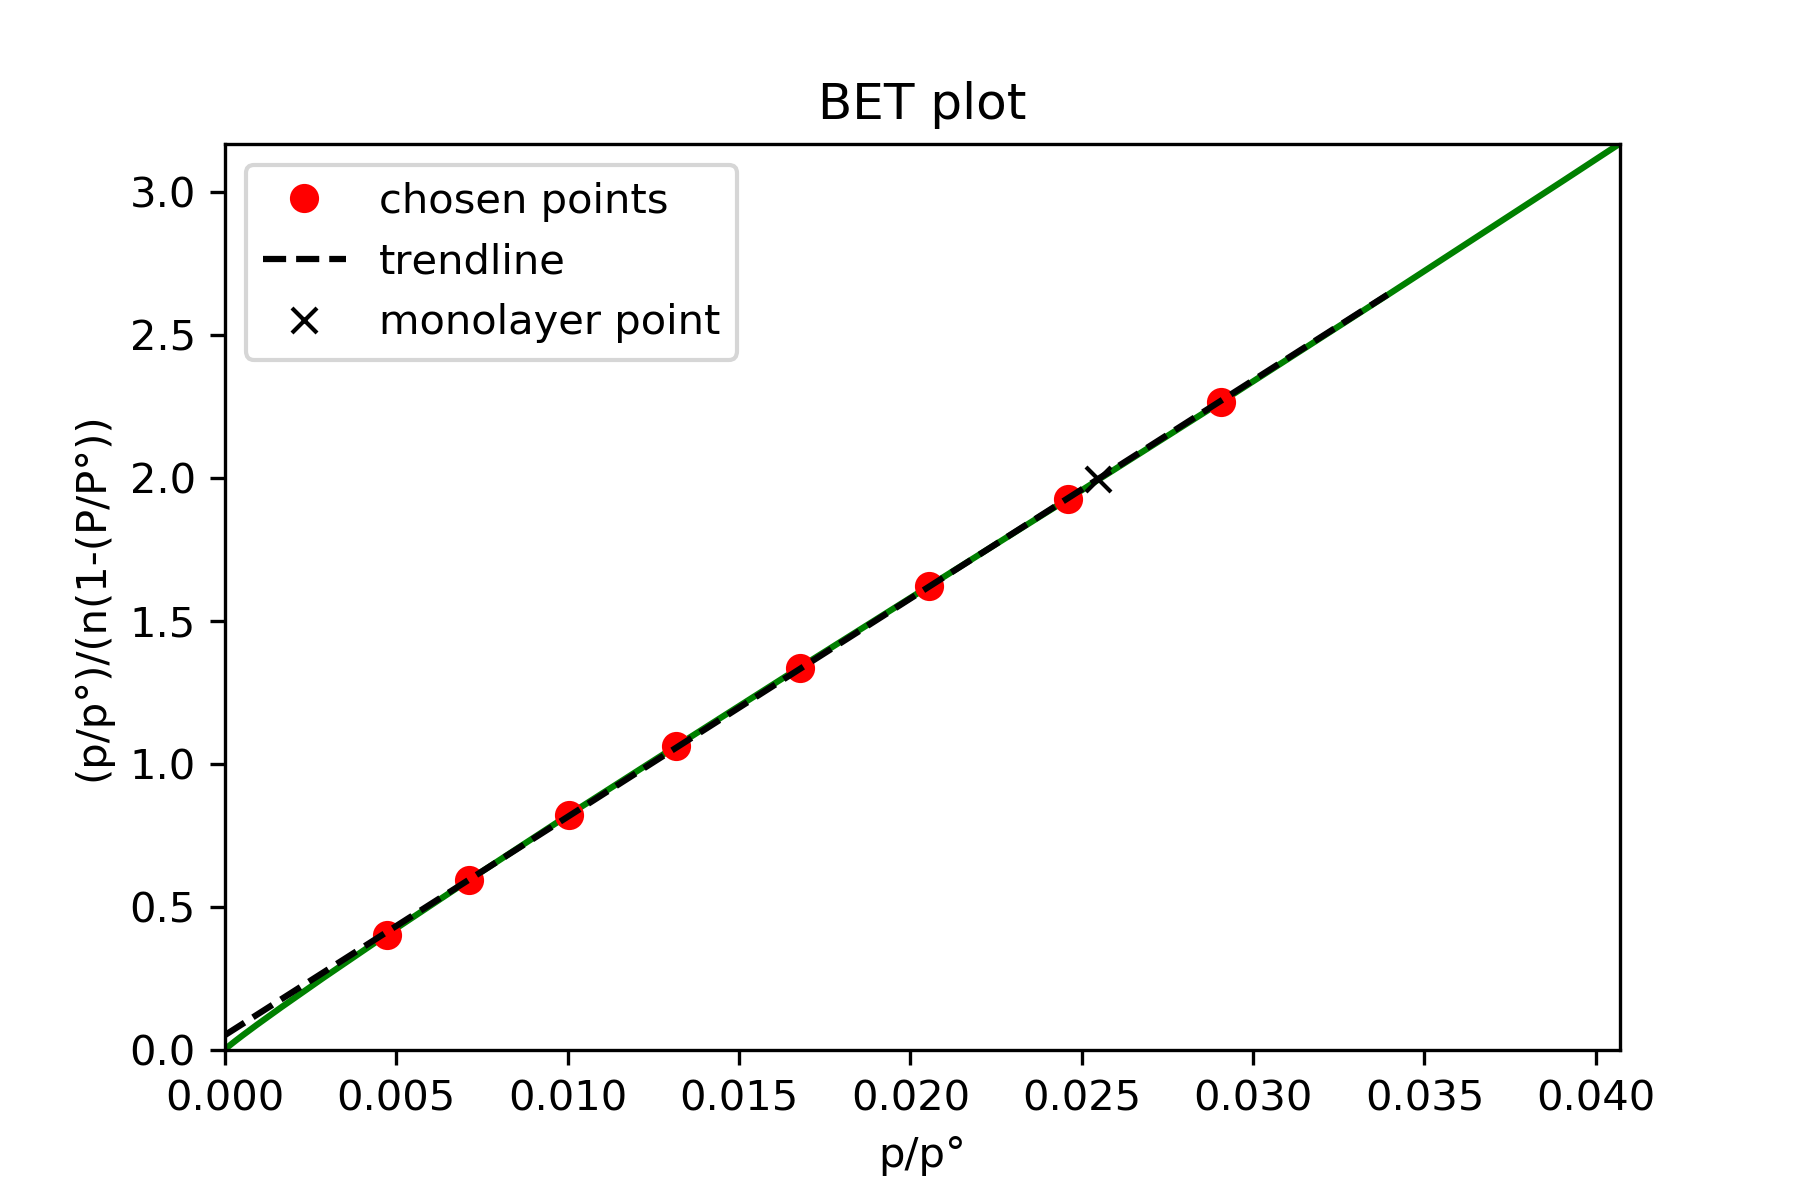
\includegraphics[width=\textwidth]{characterization/bet-plt}}
    \end{subfigure}
    \begin{subfigure}{0.4\linewidth}
        \parbox[c]{0.1\linewidth}{\caption{}%
            \label{pyg:fgr:betarea-roq}}
        \parbox[b]{0.7\linewidth}{%
            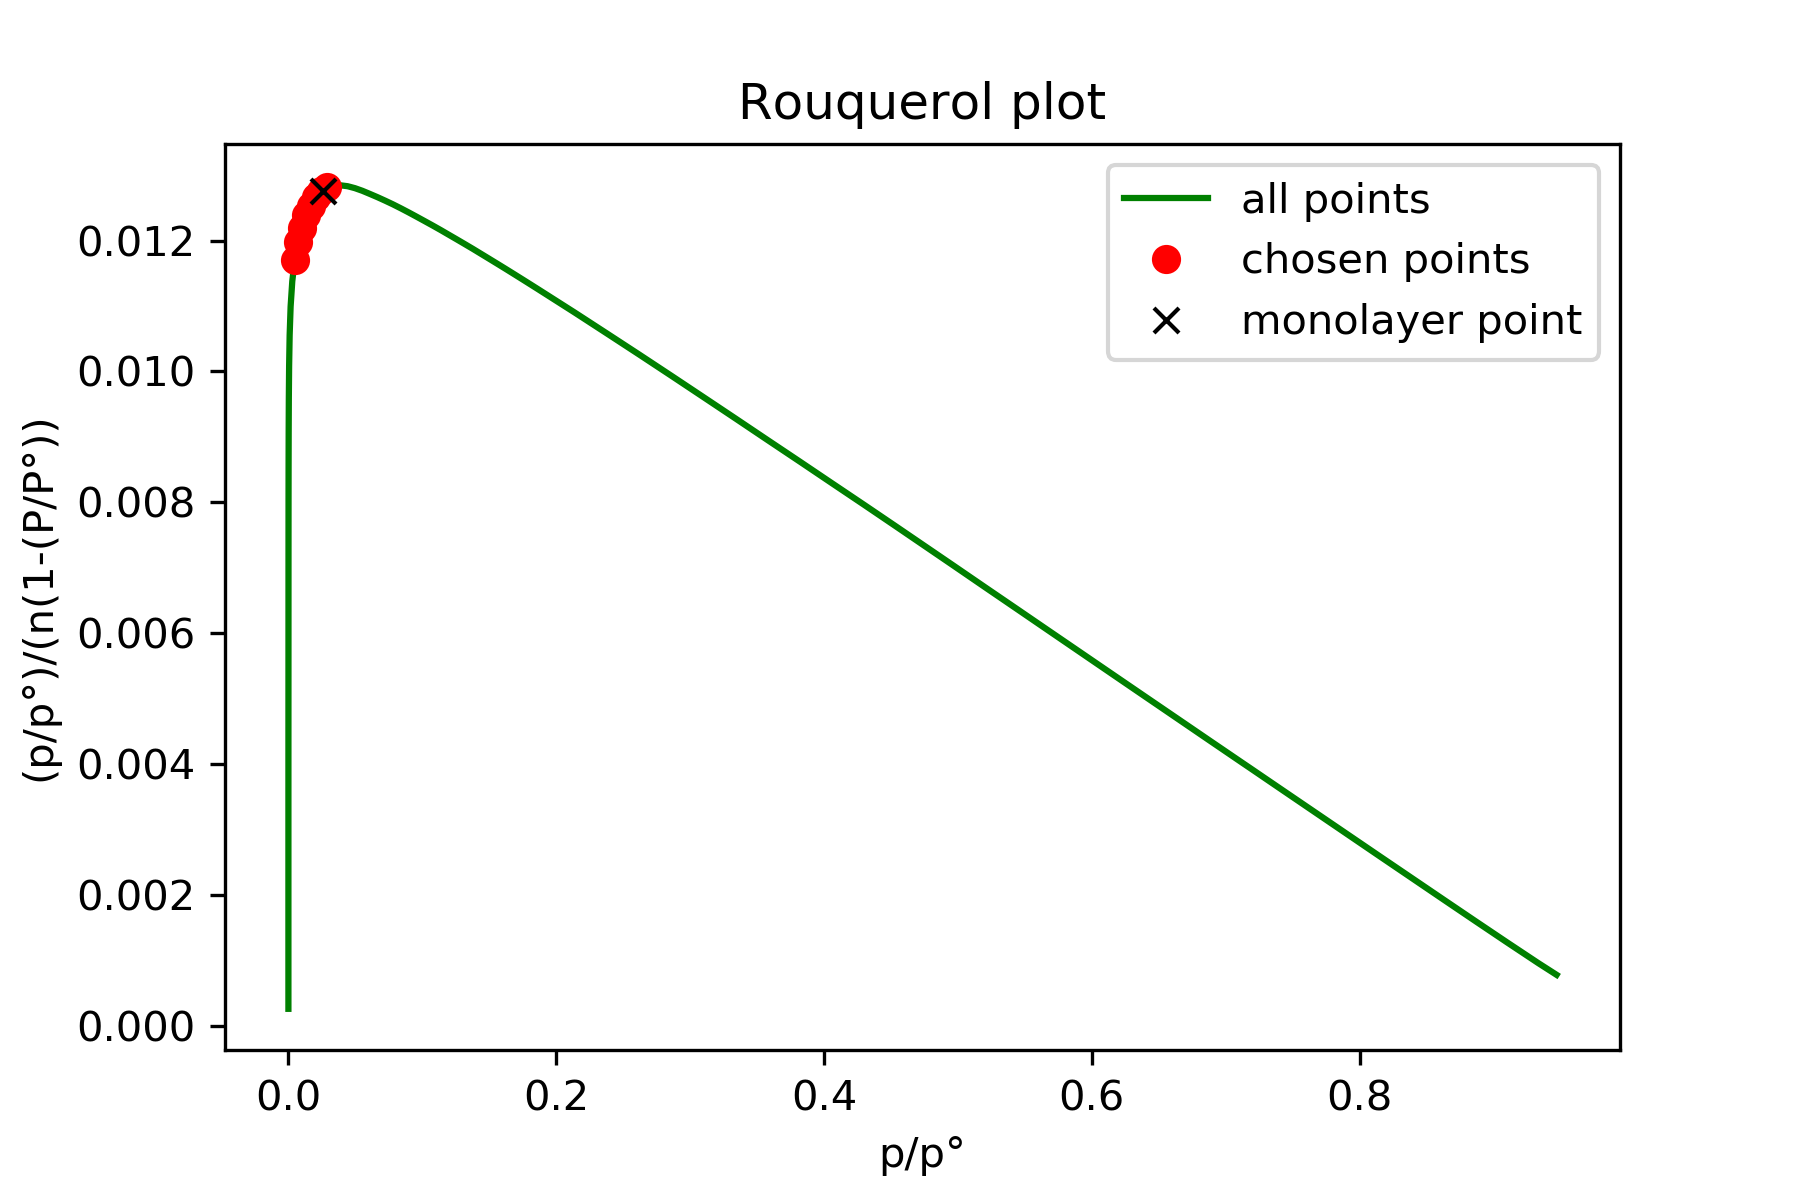
\includegraphics[width=\textwidth]{characterization/bet-roq}}
    \end{subfigure}

	\caption{Output from the BET area function (a) the BET plot showing 
	the selected points for fitting the equation, as well as the location
	of the statistical monolayer and (b) the Rouquerol plot for this 
	calculation.}%
    \label{pyg:fgr:betarea}

\end{figure}

\subsubsection{Langmuir surface area}\label{pyg:charac:langmuirarea}

The Langmuir equation (\ref{pyg:eqn:langmuir}) can be also 
be expressed in a linear form by rearranging it as:

\begin{equation}
	\frac{p}{n} = \frac{1}{K n_m} + \frac{p}{n_m}
\end{equation}

Assuming the data can be fitted with a Langmuir model, by plotting
\({P}/{n}\) against pressure, a line will be obtained. The slope and
intercept of this line can then be used to calculate \(n_{m}\),
the amount adsorbed at the monolayer, as well as \(K\), the Langmuir constant.

\begin{align}
	n_m &= \frac{1}{s} & K &= \frac{1}{i * n_m}
\end{align}

The surface area can then be calculated by using the moles adsorbed at the
monolayer using the same assumptions as when obtaining the BET surface area.

\begin{equation}
	a_{Langmuir} = n_m A_N \sigma
\end{equation}

The Langmuir method for determining surface area assumes that only a single
layer is adsorbed on the surface of the material. As most adsorption processes
(except chemisorption) don't follow this behaviour, it is important to regard
the Langmuir surface area as an estimate.

As with the BET area, the Langmuir are is calculated by using the code in
Listing~\ref{pyg:lst:langmuirarea}. The framework will alert the user
if the correlation is not linear in the selected range.
Here the \lstinline{verbose=True} option prints a short
text with all the calculation variables and the Langmuir plot as seen in
Figure~\ref{pyg:fgr:langmuirarea-auto}. If desired the user can override 
automatic pressure range selection as seen in the bottom of
Listing~\ref{pyg:lst:langmuirarea}.

\begin{lstlisting}[caption={Calculating a Langmuir area},label={pyg:lst:langmuirarea}]
area_dict = pygaps.area_langmuir(isotherm, verbose=True)
# WARINING The correlation is not linear!

area_dict = pygaps.area_langmuir(isotherm, 
									limits=(0.05, 0.3), 
									verbose=True)

# Langmuir surface area: 	a = 415 m2/g
# Minimum pressure point chosen is 0.0 and maximum is 0.194
# The slope of the Langmuir line: 		s = 234.968
# The intercept of the Langmuir line: 	i = 1.607
# The Langmuir constant is:				K = 146
# Amount for a monolayer: 				n = 0.00426 mol/g
\end{lstlisting}
\todo{make a separate style for console output}

\begin{figure}[h!]
	\centering

    \begin{subfigure}{0.4\linewidth}
        \parbox[c]{0.1\linewidth}{\caption{}%
            \label{pyg:fgr:langmuirarea-auto}}
        \parbox[b]{0.7\linewidth}{%
            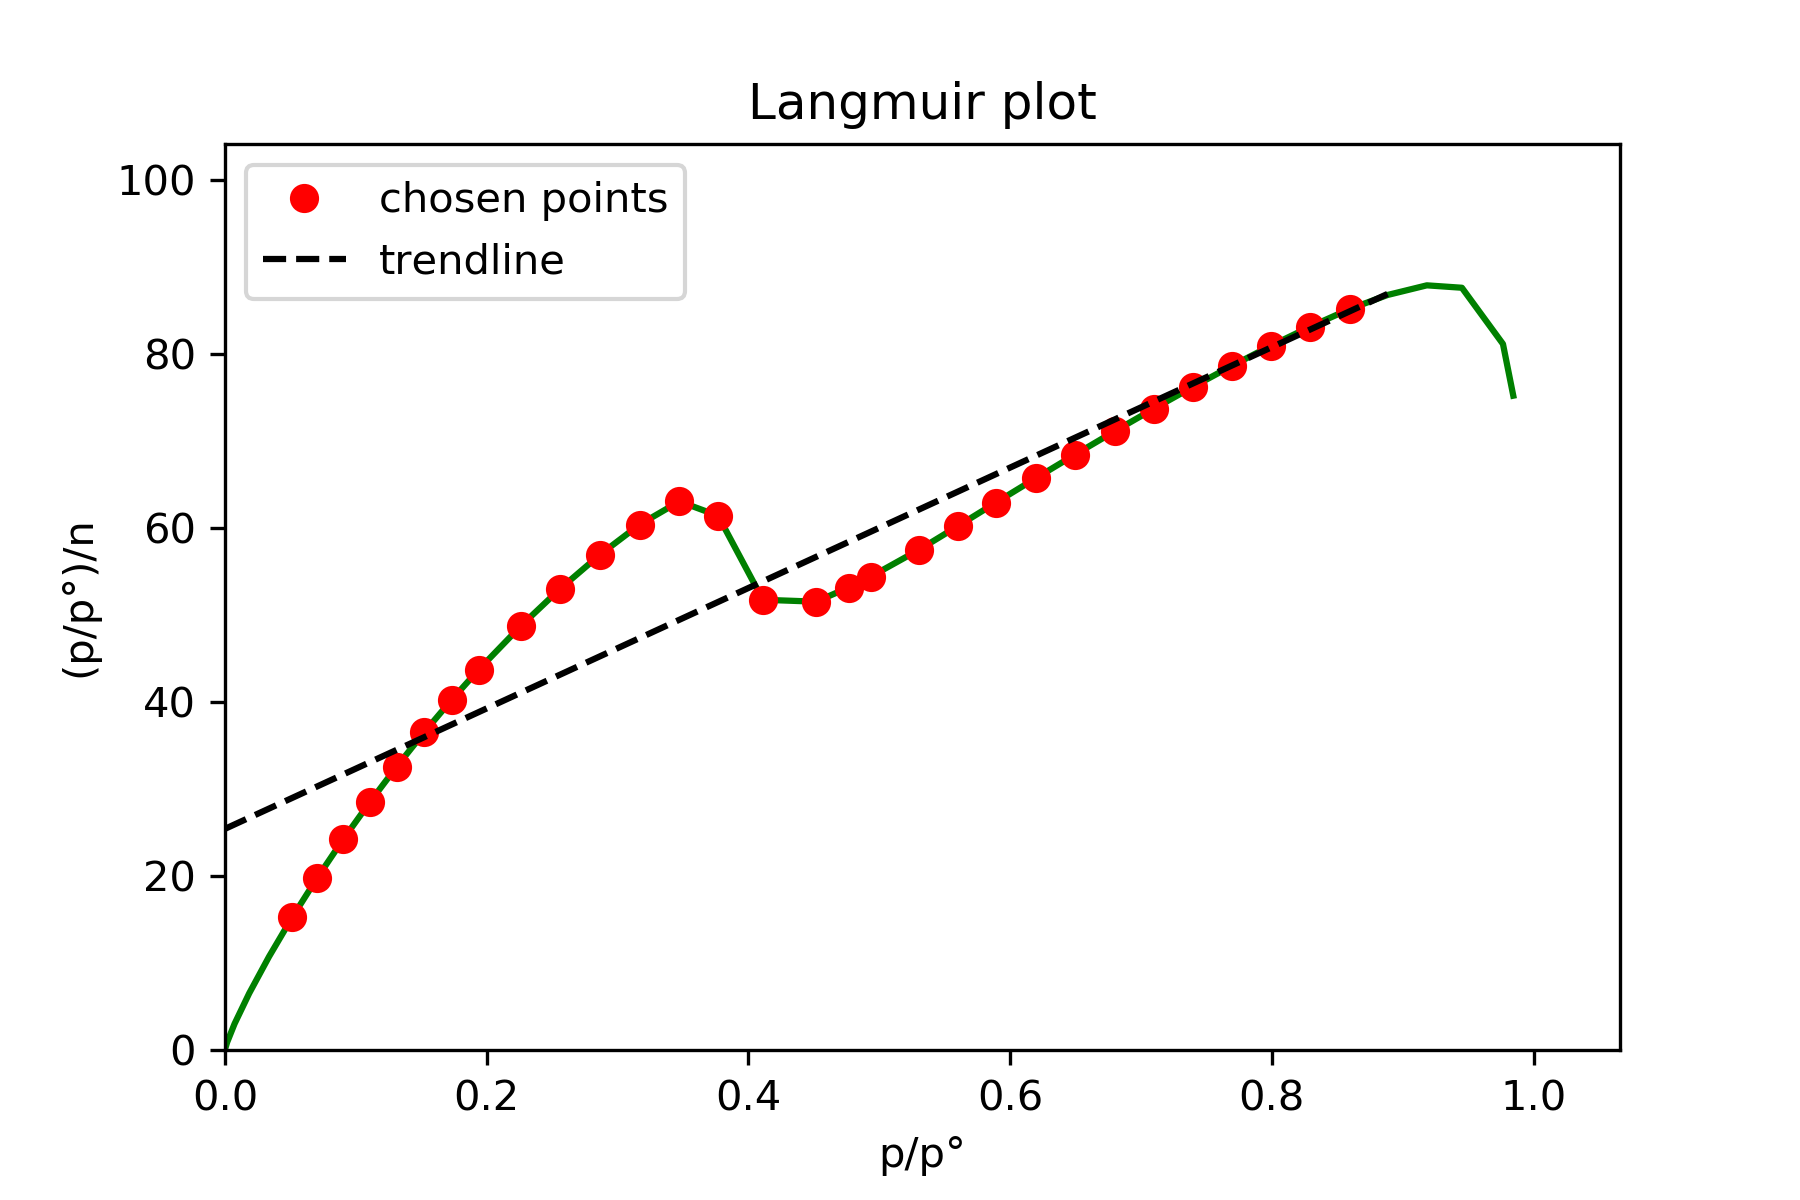
\includegraphics[width=\textwidth]{characterization/langmuir-auto}}
    \end{subfigure}
    \begin{subfigure}{0.4\linewidth}
        \parbox[c]{0.1\linewidth}{\caption{}%
            \label{pyg:fgr:langmuirarea-manual}}
        \parbox[b]{0.7\linewidth}{%
            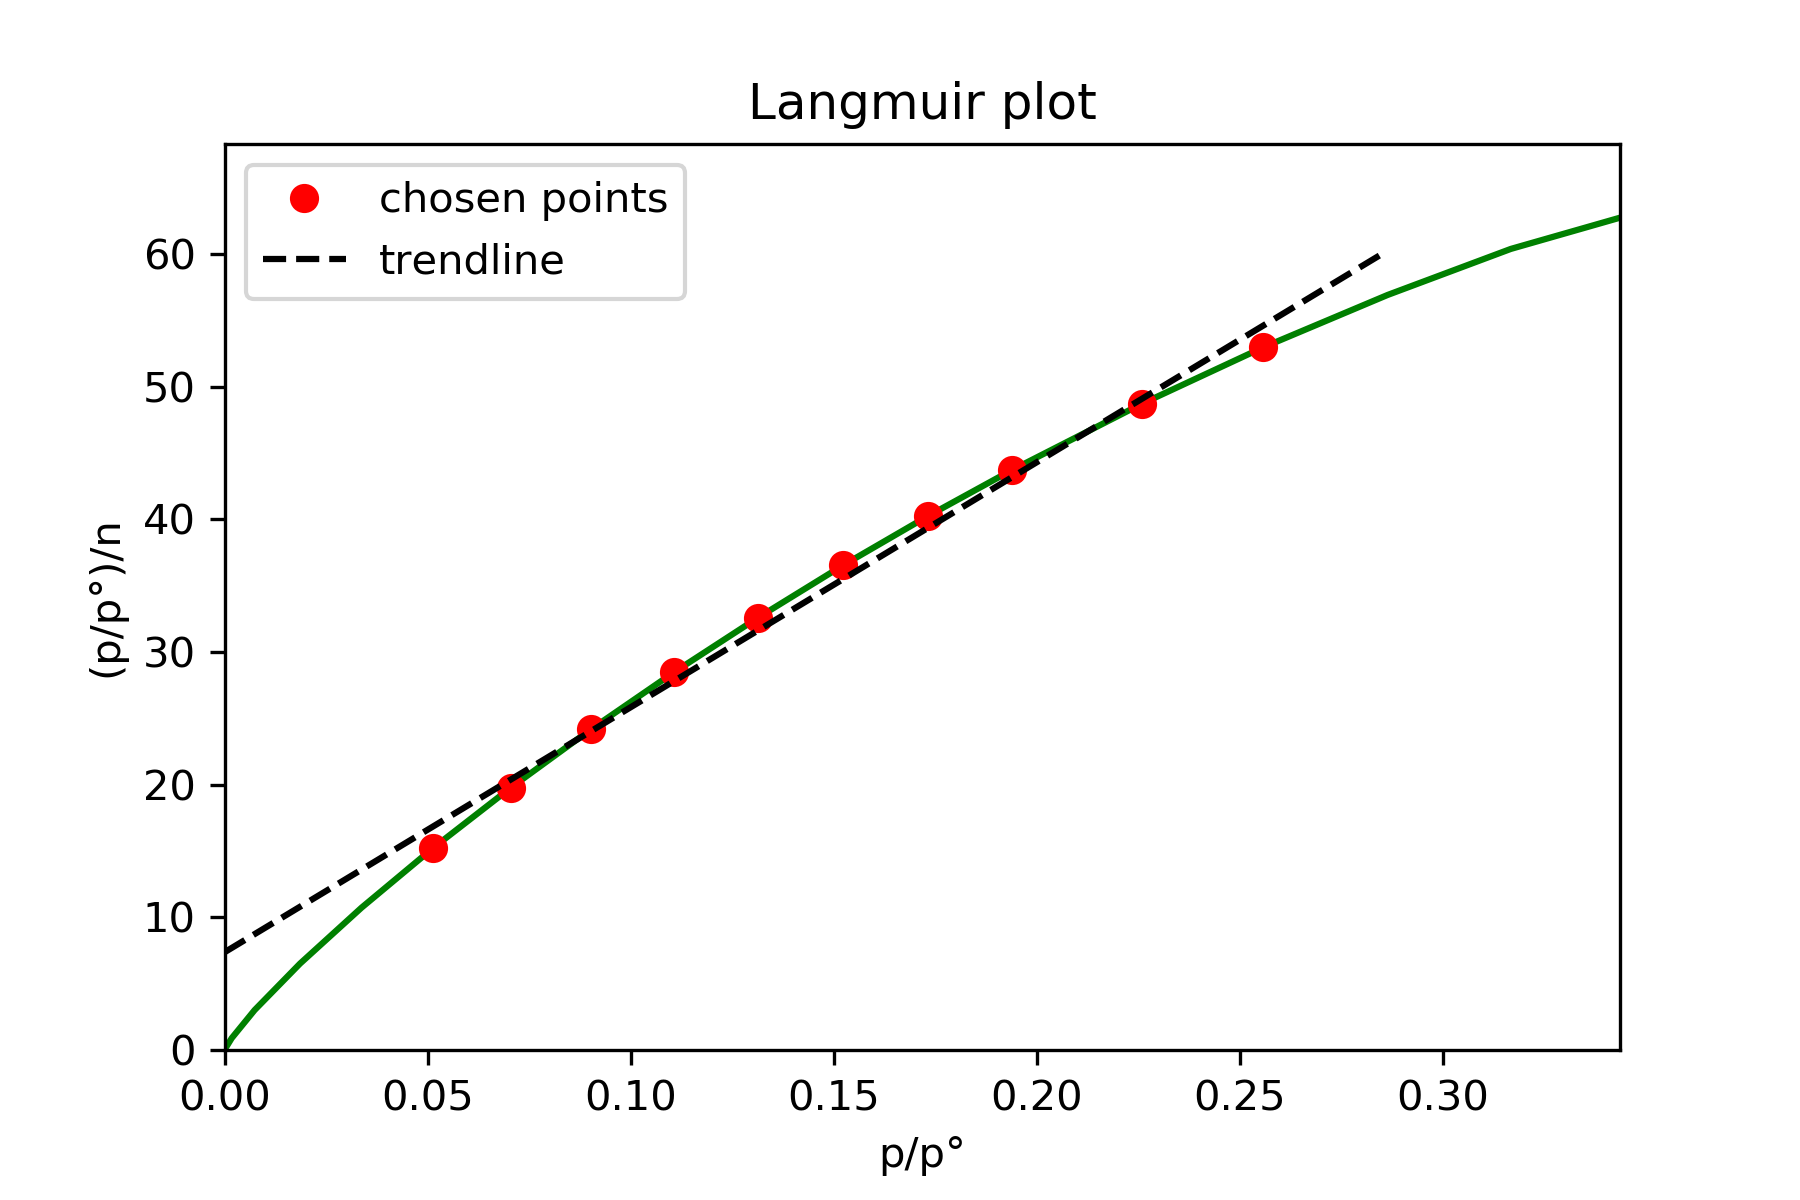
\includegraphics[width=\textwidth]{characterization/langmuir-manual}}
    \end{subfigure}

	\caption{Output from the Langmuir area function (a) the Langmuir plot 
	showing the automatic fitting attempt which generates a warning and (b) a manually
	selected pressure range for the Langmuir plot.}%
    \label{pyg:fgr:langmuirarea}

\end{figure}

\subsubsection{Ideal isotherms or thickness functions}\label{pyg:charac:tcurve}

The initial part of an isotherm (the Henry regime) can be seen to 
be very dependent on the interactions between the adsorbate and the
surface. However, the subsequent layers are less influenced by the
initial layer and can often be assumed, like in the BET model, 
to have an energy of adsorption identical to the enthalpy of liquefaction
of the bulk liquid and whose formation depends essentially only on 
the partial pressure.

With this assumption, several studies have been focused on obtaining
a reference isotherm for adsorption on a non-porous material which can
then, if the cross-sectional area of the molecule is known, be transformed
in a function capable of predicting the multilayer adsorbate thickness
as a function of pressure. This empirical function, also referred to as a
\textit{thickness function} or \textit{t-curve}, can then be used as an 
alternative method for surface area determination, as explained in 
the next section. These curves are also used in the classical methods 
for calculating mesoporous size distributions. It is important to 
clarify that the function is only applicable for a single adsorbent
and a single temperature. 

Several common thickness functions have been implemented in pyGAPS,
applicable for nitrogen at \SI{77}{\kelvin}
such as the Halsey~\cite{halseyPhysicalAdsorptionNon1948} 
(equation~\ref{pyg:eqn:halsey}) and the
Harkins and Jura~\cite{harkinsSurfacesSolidsXIII1944a}
(equation~\ref{pyg:eqn:harkinsjura}) curves.

\todo{check equations}
\begin{align}
	t_{Halsey} &= 0.354 {\Big(\frac{-5}{\log(p/p_0)}\Big)}^{1/3} \label{pyg:eqn:halsey} \\
	t_{Harkins\&Jura} &= {\Big(\frac{0.1399}{0.034 - \log_{10}(p/p_0)}\Big)}^{1/2} \label{pyg:eqn:harkinsjura}
\end{align}

These t-curves are selected by name as parameters in 
the functions that use them. The user can also define their 
own t-curve as a function and pass it as a parameter. An example
is shown in Listing~\ref{pyg:lst:tcurve} in the t-plot section.

\subsubsection{t-plot Method}\label{pyg:charac:tplot}

The t-plot method is an empirical method, developed as a
tool to determine the surface area of porous materials,
which can also be used for other calculations, such as 
external pore area and micropore volume 
calculations~\cite{lippensStudiesPoreSystems1965}.
A plot is constructed, where the isotherm loading
data is plotted versus the ideal thickness of the adsorbate layer,
obtained through the a t-curve (\ref{pyg:charac:tcurve}).
It stands to reason that, in the case when the experimentally measured
loading follows the model, a straight line will be obtained with its
intercept through the origin. However, since in most cases there
are differences between adsorption in the pores and ideal surface
adsorption, the t-plot will deviate and form features which can
be analysed to describe the material characteristics.

\begin{itemize}

	\item A sharp vertical deviation will indicate condensation
	      in a type of pore.
	\item A gradual slope will indicate adsorption on the
		  wall of a particular pore.

\end{itemize}

The slope of the linear section can be used to calculate the area where
the adsorption is taking place. If it is of a linear region at the start
of the curve, it will represent the total surface area of the material.
If at the end of the curve, it will instead represent external surface
area of the sample. The formula to calculate the area is
where \(\rho_{l}\) is the liquid density of the adsorbate at experimental
conditions

\begin{equation}
	A = \frac{s M_m}{\rho_{l}}
\end{equation}

If the region selected is after a vertical deviation, the intercept of the line
will no longer pass through the origin. This intercept be used to calculate the
pore volume through the following equation:

\begin{equation}
	V_{ads} = \frac{i M_m}{\rho_{l}}
\end{equation}

Since the t-plot method is representing a difference between the
isotherm and a model, care must be taken to ensure that the model
actually describes the thickness of a layer of adsorbate on the
surface of the adsorbent. This is more difficult than it
appears as no universal thickness curve exists.
When selecting a thickness model, make sure that it is applicable
to both the material and the adsorbate.
Interactions at loadings that occur on the t-plot lower than the monolayer
thickness do not have any physical meaning.

When the function is called without any other parameters, 
the framework will attempt to find plateaus in the data and 
automatically fit them with a straight line, returning a dictionary
with the slope, intercept and calculated pore volume and specific area
for each region fitted. As an example, the first function in
Listing~\ref{pyg:lst:tplot} will generate the graph in 
Figure~\ref{pyg:fgr:tplot-auto}. The isotherm in this example is measured
on a sample of MCM-41.

\begin{lstlisting}[caption={Generating a t-plot},label={pyg:lst:tplot}]
# using automatic region detection
pygaps.t_plot(isotherm, verbose=True)

# specifying a manual region
pygaps.t_plot(isotherm, limits=(0.3,0.44), verbose=True)

# using the Halsey thickness curve
pygaps.t_plot(isotherm, thickness_model='Halsey', verbose=True)

# defining a custom t-curve to use in the t-plot
def carbon_model(relative_p):
	return 0.88*(relative_p**2) + 6.45*relative_p + 2.98

pygaps.t_plot(isotherm, thickness_model=carbon_model, verbose=True)
\end{lstlisting}

\begin{figure}[h!]
	\centering

    \begin{subfigure}{0.4\linewidth}
        \parbox[c]{0.1\linewidth}{\caption{}%
            \label{pyg:fgr:tplot-auto}}
        \parbox[b]{0.7\linewidth}{%
            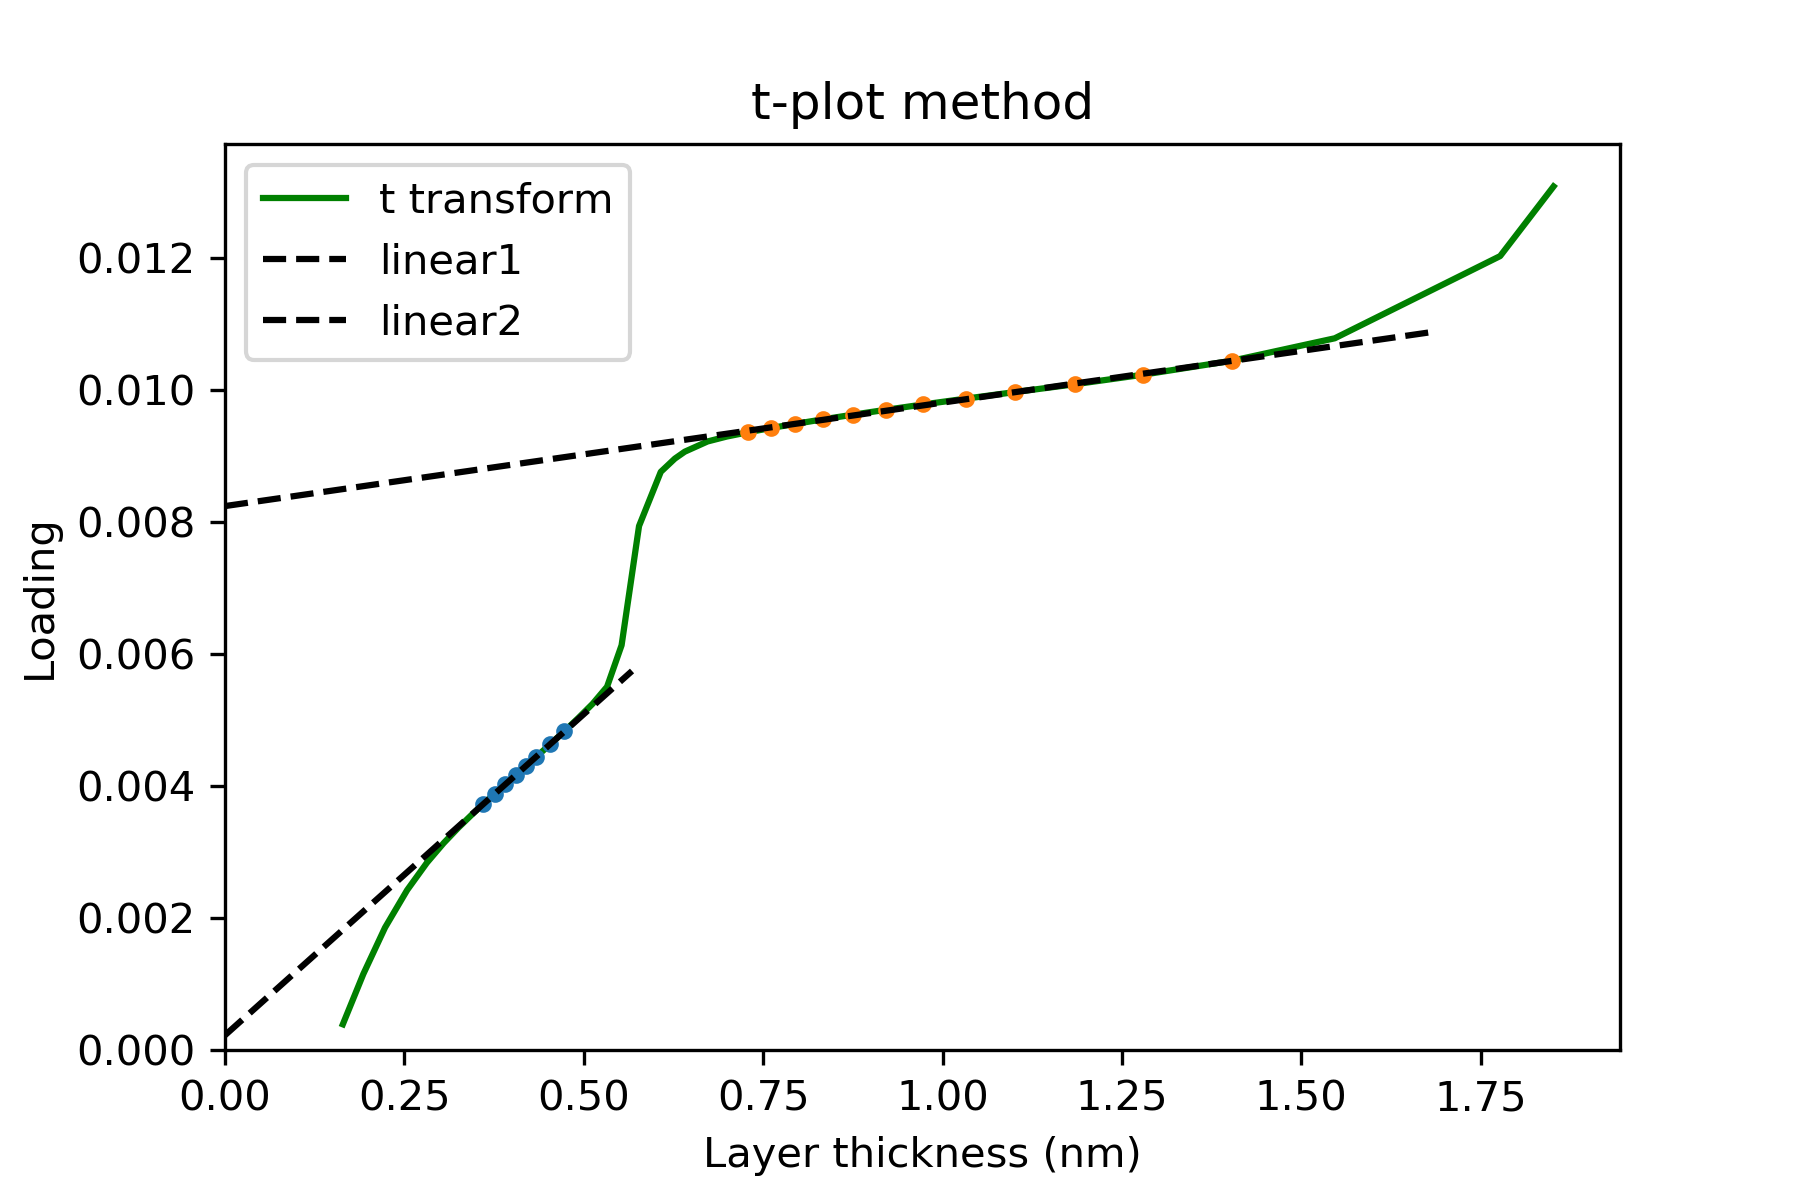
\includegraphics[width=\textwidth]{characterization/tplot-auto}}
    \end{subfigure}
    \begin{subfigure}{0.4\linewidth}
        \parbox[c]{0.1\linewidth}{\caption{}%
            \label{pyg:fgr:tplot-manual}}
        \parbox[b]{0.7\linewidth}{%
            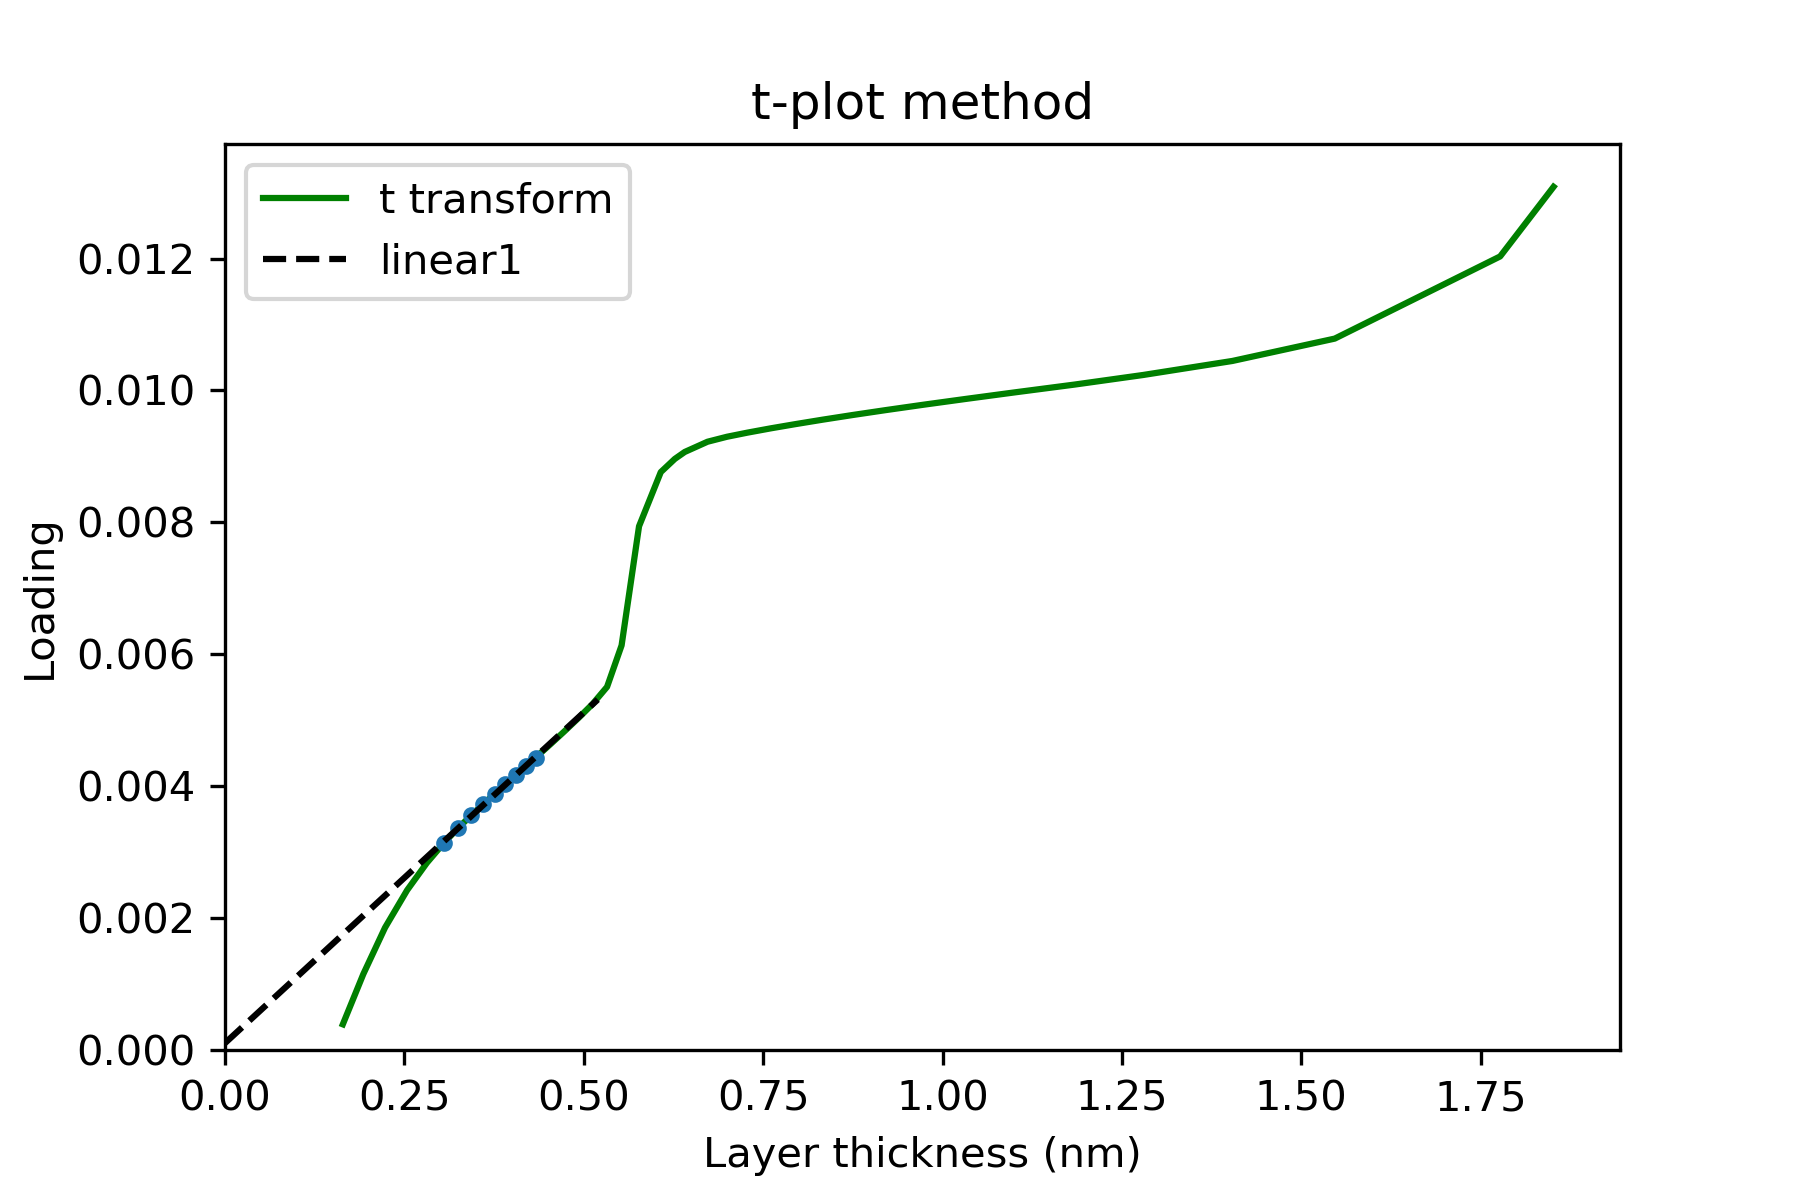
\includegraphics[width=\textwidth]{characterization/tplot-manual}}
    \end{subfigure}

	\caption{Output from the t-plot method function (a) an automatically 
	obtained t-plot with the calculated fit regions and (b) a manually
	selected range for the t-plot.}%
    \label{pyg:fgr:tplot}

\end{figure}

The first line in Figure~\ref{pyg:fgr:tplot-auto} can be attributed 
to adsorption on the pore surface, 
while the second one is adsorption on the external surface after mesopore 
filling. Two values are calculated for each section detected: the adsorbed
volume and the corresponding surface area. In this case, the area of the 
first linear region corresponds to the mesopore area. 

We can obtain a more accurate result for the surface area by 
fitting the first linear region to a zero intercept by using the 
manual region selection. Finally,
the framework allows for the thickness model to be substituted 
with an user-provided function which will be used for the thickness 
calculation, as mentioned in the t-curve section (\ref{pyg:charac:tcurve}).
A carbon black-type thickness curve is used here.

\subsubsection{\(\alpha_s\) Method}\label{pyg:charac:alphasplot}

In order to extend the t-plot analysis with other adsorbents and non-standard
thickness curves, the \(\alpha_s\) method was 
devised~\cite{atkinsonAdsorptivePropertiesMicroporous1984}.
Instead of attempting to find an ideal isotherm that describes the 
thickness of the adsorbed layer, a reference isotherm is used.
This isotherm is measured on a non-porous version of the material,
with the same surface characteristics and with the same gas.
The dimensionless \(\alpha_s\) values are obtained from this isotherm by 
dividing the loading values by the amount adsorbed at a specific relative
pressure, usually taken as 0.4 as nitrogen hysteresis loops 
theoretically close at this value.

\begin{equation}
	\alpha_s = \frac{n_a}{n_{0.4}}
\end{equation}

The analysis then proceeds as in the t-plot method. 
The slope of the linear section can be used to calculate the area
where the adsorption is taking place. If it is of a linear region
at the start of the curve, it will represent the total surface area
of the material. If at the end of the curve, it will instead
represent external surface area of the sample.
The calculation uses the known area of the reference material.

\begin{equation}
	A = \frac{s A_{ref}}{(n_{ref})_{0.4}}
\end{equation}

If the region selected is after a vertical deviation, the intercept of the line
will no longer pass through the origin. This intercept be used to calculate the
pore volume through the following equation:

\begin{equation}
	V_{ads} = \frac{i M_m}{\rho_{l}}
\end{equation}

The reference isotherm chosen for the \(\alpha_s\) method must be a description
of the adsorption on a completely non-porous sample of the same material. It is
often impossible to obtain such non-porous versions, therefore care must be 
taken how the reference isotherm is defined.

To generate an \(\alpha_s\)-plot in pyGAPS, both an analysis isotherm
and a reference isotherm must be supplied as shown in Listing~\ref{pyg:lst:alphasplot}. 
In this example, the reference isotherm is measured on non-porous silica.
The reference material area can be specified by using the \lstinline{reference_area}
parameter. If not specified, it is automatically calculated by applying the BET 
method on the reference isotherm.

\begin{lstlisting}[caption={Generating an \(\alpha_s\)-plot},label={pyg:lst:alphasplot}]
pygaps.alpha_s(isotherm, 
				reference_isotherm=isotherm_r,
				verbose=True)
\end{lstlisting}

\begin{figure}[h!]
	\centering

	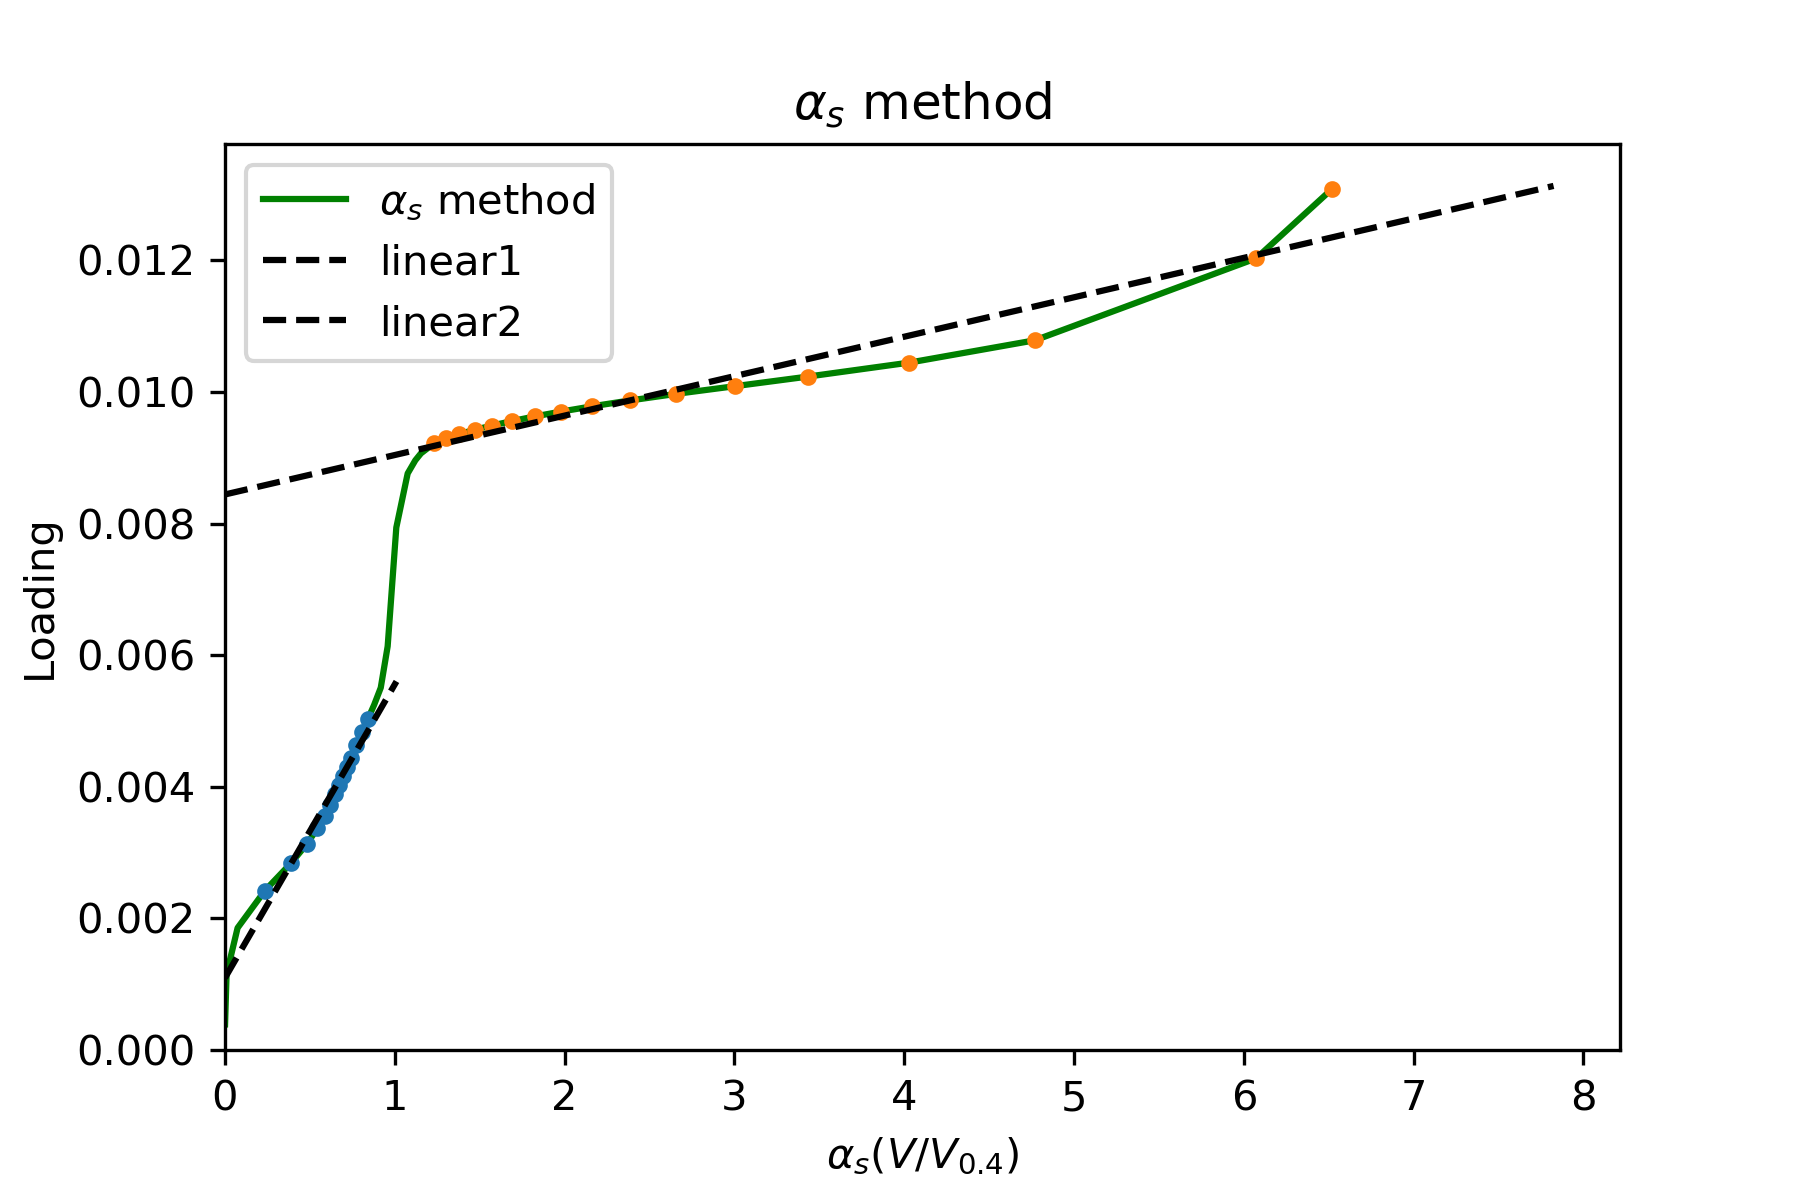
\includegraphics[width=0.4\linewidth]{characterization/alphas-auto}
	\caption{Output from the \(\alpha_s\)-plot function showing two
	automatically fit regions.}%
    \label{pyg:fgr:alphasplot}

\end{figure}
